\section{Results}
\label{sec:results}

Figure \ref{fig:atlanticbaltic} shows a comparison between numerical and analytical meridional profile of a wave travelling along a southern boundary in the Atlantic ocean (upper) and Baltic sea (lower). In both scenarios, the numerical solution underestimate the sea surface height, rapidly decaying away from the boundary.
	\begin{figure}[htbp]
		\centering
		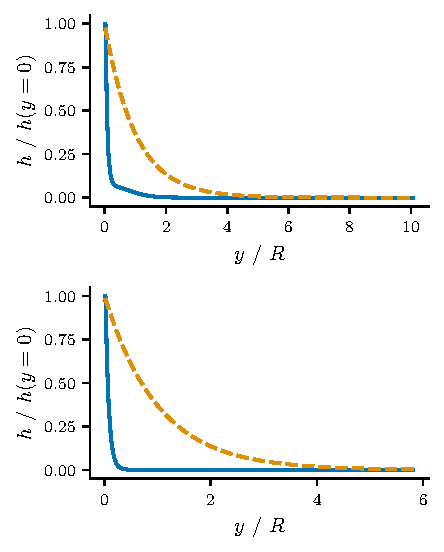
\includegraphics{slice}
		\caption{Meridional component of coastal Kelvin wave. Upper - Atlantic ocean: $ L=10^7 $ m and $D_0 = 1000$ m. Lower - Baltic sea: $ L = 10^6 $m and $ D_0 = 30 $ m. The dashed line is an analytical solution, while the solid line is numerical.}
		\label{fig:atlanticbaltic}
	\end{figure}

The time evolution of the waves at the southern boundary are shown in Figures \ref{fig:atlantic} (Atlantic ocean) and \ref{fig:baltic} (Baltic sea). A red linear line denotes a visually placed linear regression which slope is the velocity of the wave. The phase velocities are tabulated in Table \ref{tab:velocities} alongside the phase velocity of the equatorial wave. We can also see that the wave travels relatively faster in the Baltic sea, completing almost two transects compared to the one transect in the Atlantic ocean.
	\begin{figure}[htbp]
		\centering
		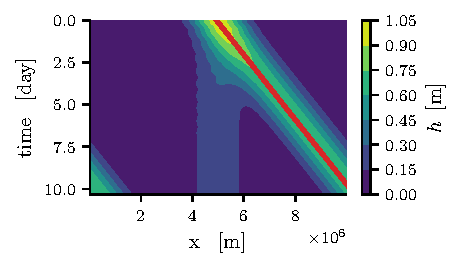
\includegraphics{hovmuller_atlantic}
		\caption{Hovmöller diagram at the equator (y=0) showing time evolution of a coastal Kelvin wave in the Atlantic ocean over 10 days. Red line represents a visually placed slope $x = 5.2 \cdot 10^5 \qty(t + 9.5)$.}
		\label{fig:atlantic}
	\end{figure}

	\begin{figure}[htbp]
		\centering
		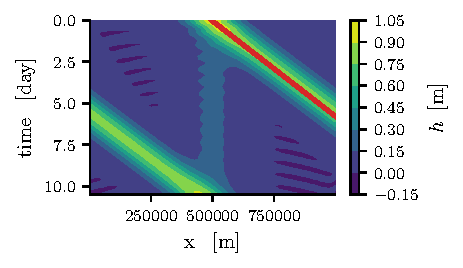
\includegraphics{hovmuller_baltic}
		\caption{Hovmöller diagram at the equator (y=0) showing time evolution of a coastal Kelvin wave in the Baltic sea over 10 days. Red line represents a visually placed slope $x = 8.7 \cdot 10^4\qty(t + 5.7)$.}
		\label{fig:baltic}
	\end{figure}

Initial and final states of an gaussian perturbation centered at the equator for a beta plane is shown in Figure \ref{fig:initialfinal_equatorial}. We see that the initial state evolves into at least two waves travelling in opposite directions. The wave travelling eastward is propagating faster and reachers the eastern boundary, splitting in two. We identify this as an equatorial Kelvin wave, agreeing with theory in propagation direction and velocity (Table \ref{tab:velocities}). In an animation, it is possible to see that some of the wave reflects, taking on a similar shape to the large westward wave.
	\begin{figure}[htbp]
		\centering
		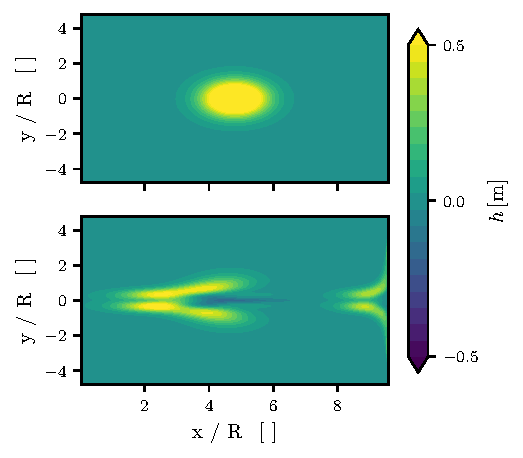
\includegraphics{initialfinal_equatorial}
		\caption{Upper - initial sea state of an equatorial perturbation. Lower - final sea state of an equatorial perturbation.}
		\label{fig:initialfinal_equatorial}
	\end{figure}
which can also be seen in Figure \ref{fig:equatorial}, where the slope in the Hovmöller diagram is steeper for the westward waves.
	\begin{figure}[htbp]
		\centering
		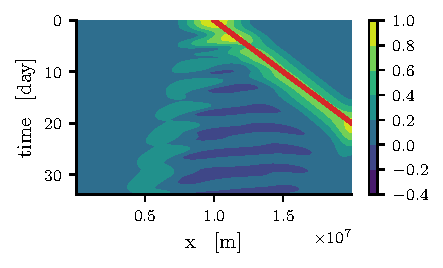
\includegraphics{hovmuller_equatorial}
		\caption{Hovmoller diagram at the equator (y=0) showing time evolution of an equatorial Kelvin wave over 35 days. Red line represents a visually placed slope $5 \cdot 10^5\qty(t + 20)$.}
		\label{fig:equatorial}
	\end{figure}

	\begin{table}[htbp]
		\begin{tabular}{lll}
			\textbf{Scenario} &\textbf{$u_{\text{num}} \, [\text{m}\text{s}^{-1}]$} & \textbf{$ u_{\text{an}} \, [\text{m}\text{s}^{-1}]$} \\
			Atlantic & $ 6.0 $ & $ 6.3 $ \\
			Baltic & $ 1.0 $ & $ 1.1 $ \\
			Equatorial & $ 5.8 $ & $ 6.3 $
		\end{tabular}
		\caption{Numerical and analytical values of phase velocities for three Kelvin wave scenarios.}
		\label{tab:velocities}
	\end{table}